\documentclass[main.tex]{subfiles}
\begin{document}
\section{Ramsey Theory}
\begin{recall*}
  For $t\geq 3$ there are graphs on $n$ vertices and approximately
  $\half\binom n 2$ edges with no $K_t$.
\end{recall*}
However, in the case of $K_{\frac n 2,\frac n 2}$, the complementary graph
would have very large cliques.
\begin{definition*}[$R(s,t)$]
  For $s,t\geq 1$, let \vocab[R(s,t)@\2]{$R(s,t)$} denote the minimum $n$ such
  that for every [not-necessarily proper] red-blue colouring of $E(K_n)$,
  there is either a $K_t$-subgraph with all edges red, or a $K_t$-subgraph with
  all edges blue.
\end{definition*}
We note that this definition is potentially undefined, because it implicitly
assumes that there exists such an $n$.
We can get around this by taking the minimum over $\bN\cup\{\infty\}$ and setting
$R(s,t) = \infty$ if no such $n$ exists (spoilers: it always will).

We have the following examples.
\begin{example*}
  \listhack
  \begin{itemize}
    \item $R(s,t) = R(t,s)$;
    \item $R(1,t) = 1$ (every edge is vacuously red);
    \item $R(2,t) = t$ for $t\geq 2$;
    \item $R(3,3) = 6$. The proof that $R(3,3) > 5$ is given by
      \begin{center}
        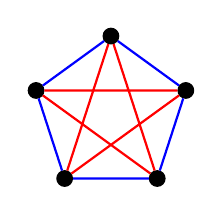
\begin{tikzpicture}
          \foreach \x in {0,...,4} {
            \node[draw, circle, fill=black, inner sep=2pt]
                at ({sin(360 * \x / 5)}, {cos(360 * \x / 5)}) (\x) {};
          }
          \draw[blue, thick] (0) -- (1) -- (2) -- (3) -- (4) -- (0);
          \draw[red, thick] (0) -- (2) -- (4) -- (1) -- (3) -- (0);
        \end{tikzpicture}
      \end{center}
  \end{itemize}
\end{example*}
We can now show that the Ramsey numbers are always finite.
\begin{proposition}
  $R(s,t)\leq R(s-1,t) + R(s,t-1)$ for all $s,t\geq 2$.
\end{proposition}
\begin{proof}
  Consider some red-blue colouring of $E(K_n)$, where $n = R(s-1,t) + R(s,t-1)$.
  Let $x\in V(K_n)$ be arbitrary, and $R_x = \{y : xy\text{ is red}\}$ and
  $B_x = \{y : xy\text{ is blue}\}$.
  Then $|R_x| + |B_x| = n - 1$.
  Since $R(s-1,t) + R(s,t-1) - 1 = |R_x| + |B_x|$,
  we either have $|R_x|\geq R(s-1,t)$ or $|B_x|\geq R(s,t-1)$.

  If $|R_x|\geq R(s-1,t)$, then the subgraph $G[R_x]$ contains either a red
  $K_{s-1}$ or blue $K_t$.
  Possibly adding $x$ gives a red $K_s$ or blue $K_t$ in $G$.
  If $|B_x|\geq R(s,t-1)$, then a symmetric argument gives either a red $K_s$
  or blue $K_t$ in $G$.
\end{proof}
\begin{corollary}
  $R(s,t)\leq 2^{s+t}$.
\end{corollary}
\begin{proof}
  Simple proof by induction; left as an exercise to the reader.
\end{proof}
\begin{theorem}
  $R(s,t)\leq\binom{s+t-2}{s-1}$ for all $s,t\geq 1$.
\end{theorem}
\begin{proof}
  Trivial if $s = 1$ or $t = 1$.
  Proceed by induction on $s+t$.
  Then
  \begin{align*}
    R(s,t)&\leq R(s-1,t) + R(s,t-1) \\
          &\leq\binom{s-1+t-2}{s-2} + \binom{s+t-3}{s-1}\tag{inductive hypothesis} \\
          &= \binom{s+t-2}{s-1}. \tag*{\qedhere}
  \end{align*}
\end{proof}
\begin{fact*}
  \listhack
  \begin{itemize}
    \item $R(4,4) = 18$.
    \item $43\leq R(5,5)\leq 48$.
      The reason this is unknown is because numbers like $2^{\binom{45}{2}}$
      is too big to brute force.
    \item $102\leq R(6,6)\leq 161$.
  \end{itemize}
\end{fact*}
We can bound $R(s,s)$; from the above facts we have
\[
  R(s,s)\leq\binom{2s-2}{s-1}\approx\frac{2}{\sqrt s}\cdot 4^s
\]
by Sterling's approximation.
This bound is from 1937.
\begin{proposition}[Erd\H{o}s 1947]
  \th\label{prop:erdos-1947}
  $R(s,s)\geq\sqrt{2}^{s-1}$.
\end{proposition}
Putting the bounds together gives
\[
  \sqrt{2}^{s-1}\leq R(S,s)\leq\frac{c}{\sqrt s}4^s.
\]
These bounds were improved this year.
\begin{theorem}[Morris, Campos, Griffith, Sahasrabudhe 2023]
  $R(s,s)\leq\left(4 - \frac{1}{128}\right)^s$.
\end{theorem}

\begin{proof}[Proof of \th\ref{prop:erdos-1947}]\lecture{Tue Oct 17}%
  Suppose $n\leq\sqrt{2}^{s-1}$ (we may assume $s\geq 3$).
  It suffices to show that $K_n$ has a red-blue-colouring with no monochromatic $K_s$.

  Colour each edge o the complete graph on $[n] = \{1,\ldots,n\}$ red or blue
  independently with probability $\half$.
  For each $X\in\binom{[n]}{s}$,
  \begin{align*}
    \bP(X\text{ is monochromatic})
    &= \bP(X\text{ is red}) + \bP(X\text{ is blue}) \\
    &= \left(\half\right)^{\binom s 2} + \left(\half\right)^{\binom s 2} \\
    &= 2^{1 - \binom s 2}.
  \end{align*}
  For each $X\in\binom{[n]}{s}$, let $C_X$ be the indicator variable for the
  event that $X$ is monochromatic.
  Then
  \[
    \bE[C_X] = \bP(X\text{ is monochromatic}) = 2^{1-\binom s 2}
  \]
  so
  \begin{align*}
    \bE[\#\text{monochromatic $s$-subsets}] = \sum_{X\in\binom{[n]}{s}}\bE[C_X]
    = \binom{n}{s}\cdot2^{1-\binom{s}{2}}
  \end{align*}
  and
  \begin{align*}
  \binom{n}{s}2^{1-\binom s 2}\leq\frac{n^s}{s!}2^{1-\binom s 2}
  \leq\frac{\sqrt{2}^{s(s-1)}}{s!} = \frac{2}{s!} < 1
  \end{align*}\mnote{While $s!$ is large, it will only give you improvements to
  lower order terms and will not improve the exponent.}
  so there exists a red-blue colouring of $K_n$ with no monochromatic $s$-sets.
\end{proof}
\subsection{Ramsey Theory With More Colours}
Let $R(s_1,s_2,\ldots,s_k)$ be the minimum $n$ (possibly infinite) such that
for each colouring of $E(K_n)$ with colours from a set $\{c_1,\ldots,c_k\}$,
there is a $K_{s_i}$ coloured $c_i$ for some $i$.

\begin{theorem}
  $R(s_1,s_2,\ldots,s_k)$ exists for all $s_1,s_2,\ldots,s_k$.
\end{theorem}
\begin{proof}[Proof Sketch for $k=3$]
  It can shown that
  \[
    R(s_1,s_2,s_3)\leq R(s-1,s_2,s_3) + R(s_1,s_2,s_3) + R(s_1,s_2,s_3-1)
  \]
  which gives $R(s_1,s_2,s_3)\leq 3^{s_1+s_2+s_3}$ so $R(s,s,s)\leq 27^s$.
\end{proof}
\begin{proof}[Alternate Proof]
  We show $R(s_1,\ldots,s_k)\leq R(s_1,\ldots, s_{k-2}, R(s_{k-1}, s_k))$.
  Suppose $n\geq R(s_1,\ldots,s_{k-2},R(s_{k-1},s_k))$ and let
  $c:E(K_n)\to\{1,\ldots,k\}$ be a $k$-colouring.
  Define $c':E(K_n)\to\{1,\ldots,k-1\}$ by
  \[
    c'(e) = \begin{cases}
      c(e) & \text{if }c(e)\leq k-1 \\
      k-1 & \text{if } c(e) = k
    \end{cases}
  \]
  that is, we merge colours $k-1$ and $k$.

  By the choice of $n$, there is either a $K_{s_i}$ of colour $i$ for some
  $i < k-1$ (with respect to $c$) or a $K_{R(s_{k-1}, s_k}$ where every edge
  has colour $k-1$ or $k$ (with respect to $c$).
  In the case, we're done.

  In the second case, applying the definition of $R(s_{k-1},s_k)$ implies a
  $K_{s_{k-1}}$ of colour $k-1$ or a $K_{s_k}$ of colour $k$.
\end{proof}
However this gives bounds
$R(s,s,s)\leq R(s,R(s,s))\leq 2^{s + R(s,s)}\leq 2^{s + 4^s}$
which is doubly exponential.

\begin{remark*}
  There is a generalization that replaces cliques with arbitrary subgraphs.
  This is called \vocab{graph Ramsey theory} and is in Diestel and very hard.
\end{remark*}

\subsection{Ramsey Theory for Tournaments}
\begin{definition*}
  A \vocab{tournament} is a complete graph with orientated edges.
\end{definition*}
By colouring all ``forward'' edges red and all ``backwards'' edges red,
Ramsey's theorem gives a subset with a linear order.

Interestingly, the Ramsey numbers for tournaments are smaller than those
for red-blue colourings of cliques.

\subsection{Ramsey Theory for Infinite Graphs}
\begin{theorem}
  Let $K$ be a complete graph with vertex set $\bN$.
  For every red-blue colouring of $E(K)$, there is a monochromatic subgraph
  isomorphic to $K$ (equivalently, an infinite monochromatic subset of $V(K)$).
\end{theorem}
\begin{proof}\mnote{One of the good things about this proof is that it
  recognizes the base case of Ramsey's theorem (when inducting on the number
  of colours) is the pigeonhole principle.}
  We prove that there is a sequence $a_0 < a_1 < a_2 < \cdots$ in $\bN$ and
  $c_0,c_1,\ldots$ in $\{\text{red}, \text{blue}\}$ and
  $N\supseteq B_0\supseteq B_1\supseteq B_2\supseteq\cdots$ such that
  \begin{itemize}
    \item for all $i\geq 0$, $|B_i| = \infty$ and $a_{i+1}\in B_{i+1}\subseteq(a_i,\infty)$;
    \item for all $i$ and all $b\in B_i$, edge $a_ib$ has colour $c_i$.
  \end{itemize}
  Choose $a_0 = 0$, $c_0$ be a colour such that infinitely many pairs $a_0x$
  have colour $c_0$, and $B_0 = \{x : a_0x\text{ has colour }c_0\}$

  Given $a_0,\ldots,a_k$, $B_0,\ldots,B_k$, $c_0,\ldots,c_k$ already chosen,
  Choose $a_{k+1} = \min(B_k), c_{k+1}, B+{k+1}$ such that $B_{k+1}\subseteq B_k$,
  $|B_{k+1}| = \infty$ and every edge from $a_{k+1}$ to $B_{k+1}$ has colour $c_{k+1}$.

  By construction, for all $i < j$,
  $a_j\in B_{j-1}\subseteq B_{j-2}\subseteq\cdots\subseteq B_i$
  so $a_ia_j$ has colour $c_i$.
  Now there is some colour $c\in\{\text{red},\text{blue}\}$ such that infinitely
  many $c_i$ are equal to $c$.
  Now $\{a_i : c_i = c\}$ is by construction an infinite set where all pairs
  have colour $c$.
\end{proof}
\begin{theorem}[K\H{o}nig's Infinity Lemma]
  Let $T$ be an infinite tree with root $r$, and ``layers''
  $X_0 = \{r\}, X_1, X_2, \ldots$ defining distance from $r$ (so each vertex
  other than $r$ has exactly one neighbour in the previous layer, and all other
  neighbours in the next layer) such that every vertex has finite degree.
  Then $T$ has an infinite path $r, x_1, x_2,\ldots$ where $x_i\in X_i$.
\end{theorem}
\begin{proof}\lecture{Thu Oct 19}%
  Call a vertex $x$ \textit{heavy} if there are infinitely many vertices $y$
  ``above it'' (i.e. $x$ is on the path from $y$ to the root).
  Since $T$ is infinite, the root is heavy.
  Since degrees are finite, each heavy vertex is adjacent to a heavy vertex in
  the layer above.
  Because of this, there exists an infinite sequence $r = x_0, x_1, \ldots$ of heavy vertices.
\end{proof}
With this lemma, we can derive finite Ramsey from infinite Ramsey.
\begin{proof}
  Assume infinite Ramsey, and suppose finite Ramsey fails for some $t\in\bN$.
  For each $n\in\bN$, let $C_n$ be the set of colourings of $E(K_{[n]})$ with
  no monochromatic $K_t$-subgraph, where $K_{[n]}$ is the complete graph with
  vertex set $[n]=\{1,2,\ldots,n\}$.
  Since Ramsey fails, we have $C_n\neq\varnothing$ for all $n$.

  Define a tree $T$ on $\bigcup_{n\geq 0} C_n$ by joining each $c\in C_i$ for
  $i > 0$ to the colouring $c'\in C_{i-1}$ obtained from $c$ by discarding the
  vertex $i$.

  \mnote{There are no cycles because if there were, the cycle would be finite,
  but the maximum vertex would then have down degree at least 2,
  which is impossible.}%
  Since $C_n\neq\varnothing$ for all $n$, and each colouring $c\in C_n$ has
  only finitely many (i.e. at most $2^n$) extensions to a colouring in $c_{n+1}$,
  this satisfies the hypotheses of K\H{o}nig's Lemma.
  So there is an infinite sequence $c_0,c_1,\ldots,$ with $c_i\in C_i$ and such
  that each $c_{i+1}$ is an extension of $c_i$ to a colouring of $K_{[i+1]}$.
  This defines a colouring $c_\infty$ of $E(K_{\bN})$ where, for $i < j$,
  $c_\infty(ij)\coloneqq c_j(ij)$ (and all subsequent colourings agree).

  By infinite Ramsey, there is a monochromatic set $X$ of set $t$ in $K_\bN$
  with respect to $c_\infty$.
  \rmnote{This is what makes the proof non-constructive,
  because you cannot bound $\max(X)$.}%
  But then $X$ is monochromatic with respect to $C_{\max(X)}$, which contradicts
  the definition of the $C_i$.
\end{proof}
There is no Ramsey theorem for uncountable graphs.
\begin{theorem}[Sierpinski]
  There exists a red-blue colouring of $K_\bR$ so that every monochromatic
  complete subgraph is countable (but you need axiom of choice).
\end{theorem}
\begin{proof}[Proof Sketch]
  Let $<_w$ be a well-ordering of $\bR$, i.e. any non-empty subset has a minimum.
  For $x < y$ (in the usual ordering), colour $xy$ blue if $x <_w y$ and red
  otherwise.
  If $X$ is monochromatic, up to flipping the usual ordering, you have a
  well-ordering on $X$, you can injectively map $X$ to $\bQ$
  (repeatedly compute $\min\{y\in X : x < y\}$) and so $X$ is countable.
\end{proof}
\subsection{Ramsey Theory for Hypergraphs}
For $k\in\bN$, let $R_k(s,t)\in\bN\cup\{\infty\}$ be the smallest $n$ such that
for all $|X| = n$ and red-blue colouring of $\binom{X}{k}$, there is either a
$s$-element set $X_0\subseteq X$ such that $\binom{X_0}{k}$ is red,
or a $t$-element set $X_0$ such that $\binom{X_0}{k}$ is blue.
\begin{theorem}[Hypergraph Ramsey]
  $R_k(s,t)$ is finite for all $k, s, t$.
\end{theorem}
\begin{proof}
  We have $R_1(s,t) = s+t-1$ (pigeonhole).
  Suppose that $k\geq 2$, and inductively assume that $R_{k-1}(s',t') < \infty$
  for all $s',t'$.

  We argue that $R_k(s,t)\leq 1 + R_{k-1}(R_k(s-1,t),R_k(s,t-1))$.
  The result will follow by induction on the value of $s+t$, since this means
  $R_k(s-1,t) < \infty, R_k(s,t-1) < \infty$ and $R_{k-1}(\cdot,\cdot) < \infty$.

  Suppose $n\geq 1 + R_{k-1}(R_k(s-1,t),R_k(s,t-1))$ and consider a colouring
  of $\binom X k$ where $|X| = n$.
  Let $v\in X$.
  Define a colouring $c'$ of $\binom{X-v}{k-1}$ by setting
  $c'(A)\coloneqq c(A\cup\{v\})$ for each $A$
  Since $|X-v|\geq R_{k-1}(R_k(s-1,t), R_k(s,t-1))$, we either have a red
  $R_k(s-1,t)$-set with respect to $c'$ or a blue $R_k(s,t-1)$-set with respect
  to $c'$.
  Suppose $X_0\subseteq X-v$ is a red $R_k(s-1,t)$-set with respect to $c'$.
  Then $X_0$ contains a red $(s-1)$ set with respect to $c$ or a blue $t$-set
  with respect to $c$.
  In the first case, adding $v$ to the set gives a red $s$-set in $X$,
  and the latter case gives a blue $t$-set in $X$.

  The other case is similar.
\end{proof}
\begin{corollary*}
  A multicoloured version $R_k(s_1,s_2,\ldots,s_t) < \infty$ for all
  $k,s_1,\ldots,s_t$.
\end{corollary*}
\begin{proof}
  Colour-merging, i.e.
  \[
    R_k(s_1,\ldots,s_t)\leq R_k(s_1,\ldots,s_{t-1}, R_k(s_{t-1},s_t)). \qedhere
  \]
\end{proof}
\subsection{Ramsey Theory for Infinity Many Colours}
\begin{question*}
  What if there is no bound on the set of colours?
\end{question*}
We have the following answer.
\begin{theorem}[Canonical Ramsey Theorem (Erd\H{o}s-Rado 1950)]
  For every function
  $f:\binom{\bN}{2}\to C$, there exists an infinite subset $X$ such that on
  $X$, either:
  \begin{itemize}
    \item $X$ is monochromatic with respect to $f$;

    \item $X$ is ``rainbow'' with respect to $f$, i.e. no two edges in
      $\binom X 2$ have the same colour;

    \item $X$ is left-homogeneous, i.e. there exists an injective function
      $\varphi:X\to C$ such that for all $x\in X$ and all $y\in X$ with $y > x$,
      $f(xy) = \varphi(x)$; or

    \item $X$ is right-homogeneous, i.e. there exists an injective function
      $\varphi:X\to C$ such that for all $x\in X$ and all $y\in Y$ with $y < x$,
      $f(xy) = \varphi(x)$.
  \end{itemize}
\end{theorem}
\begin{proof}\lecture{Tue Oct 24}%
  We first need a series of claims.
  \begin{claim}
    There is a sequence $x_0 < x_1 < \cdots$ such that for all $x_i$, either:
    \begin{enumerate}[label=(\arabic*)]
      \item There exists $c_i$ such that $f(x_ix_j) = c_i$ for all $j > i$; or
      \item $f(x_ix_j)\neq f(x_ix_{j'})$ for all $j' > j > i$.
    \end{enumerate}
  \end{claim}
  \begin{subproof}[Proof Sketch]
    Start with $x_0 = 0$; there are either infinitely many of the same colour,
    or infinitely many colours: pick the minimum to be $x_1$ and repeat via induction.
  \end{subproof}

  \begin{claim}
    There is a sequence $x_0' < x_1' < \cdots$ such that either
    \begin{enumerate}[label=\arabic*]
      \item[1(a):] (1) occurs for all $i$, with $c_0 = c_1 = c_2 = \cdots$;
      \item[1(b):] (1) occurs for all $i$, with $c_0, c_1, \ldots$, distinct; or
      \item[(2):] (2) occurs for all $i$.
    \end{enumerate}
  \end{claim}
  \begin{subproof}\mnote{Note this proof appeals to pigeonhole, i.e. Ramsey
      for size-1 subsets, so the generalization to hypergraphs follows by
    inducting on the number of vertices in each hyperedge.}%
    If (2) occurs infinitely in $x_0 < x_1 < \cdots$, take $x_i'$ to be a
    subsequence where it always occurs, giving (2).
    If (1) occurs infinitely often, it occurs either with the same $c_i$
    infinitely often, or infinitely many distinct $c_i$; taking a subsequence
    gives 1(a) or 1(b).
  \end{subproof}

  If 1(a) occurs, then $(x_i')$ is constant coloured (since
  $f(x_i'x_j') = c_i' = c_0$ for all $i < j$).
  If 1(b) occurs, then $(x_i')$ is left-homogeneous since $f(x_i'x_j) = c_i$
  for all $i < j$ and the $c_i$ are distinct.

  \rmnote{If you're only interested in finite Ramsey, you can just flip the
  sequence around at this point.}%
  So we may assume outcome (2) holds.
  Say a pair $y,y'$ \textit{concurs} with respect to a set $Z$ if
  $f(yz) = f(y'z)$ for all $z\in Z$.
  Say $y,y'$ \textit{conflict} with respect to $Z$ if $f(yz)\neq f(y'z)$
  for all $z\in Z$.

  \begin{claim*}
    There is a subsequence $y_0 < y_1 < \cdots$ of the $x_i'$ such that for all
    $i < j$, either:
    \begin{enumerate}
      \item $y_i,y_j$ concurs with respect to $\{y_{j+1},\ldots\}$; or
      \item $y_i,y_j$ conflicts with respect to $\{y_{j+1},\ldots\}$.
    \end{enumerate}
  \end{claim*}
  \begin{subproof}
    It suffices by induction to show that, for all $y_0,\ldots, y_t$ and
    $Z\subseteq (y_t,\infty)$ with $|Z| = \infty$ such that all pairs
    $(y_i,y_j)$ either all concur or conflict with respect to $Z$, there is
    some $y_{j+1}\in Z$ and an infinite subset $Z'\subseteq Z$ such that all
    pairs $y_i,y_{t+1}$ with $0\leq i\leq t$ concur or conflict with $Z'$.

    Choose $y_{t+1} = \min(Z)$.
    Then $Z - \{y_{t+1}\}$ has an infinite subset $Z_0$ such that $y_0, y_{t+1}$
    either concurs or conflicts on $Z$ (by infinite pigeonhole).
    $Z_0$ has an infinite subset $Z_0$ such that $y_1,y_{t+1}$ either concur or
    conflict on $Z_1$, and repeating $t$ times shows that $Z$ has an infinite
    subset $Z'$ such that all pairs $y_i,y+{t+1}$ concur or conflict on $Z'$.
  \end{subproof}
  By Ramsey's theorem for infinite 2-coloured graphs, there is an infinite
  subsequence $z_0 < z_1 < \cdots$ of the $y_i$ such that either
  \begin{enumerate}[label=2(\roman*)]
    \item all pairs $z_i,z_j$ with $i < j$ concur on $\{z_{j+1},\ldots\}$; or
    \item all pairs $z_i,z_j$ with $i< j$ conflict on $\{z_{j+1},\ldots\}$.
  \end{enumerate}
  If 2(i) holds, then since $z_i$ is a subsequence of $x_i$, we have
  $f(z_iz_j)\neq f(z_iz_k)$ and $f(z_iz_k) = f(z_jz_k)$ for all $i < j < k$.
  It is left as an exercise to the reader than $z_i$ is right-homogeneous.

  If 2(ii) holds, then let $(w_0,\ldots,w_t)$ be a rainbow set.
  There are exactly $\binom{t+1}(2)$ colours occurring in the pairs $w_iw_j$,
  and each vertex in the $w_i$ has at most 1 right neighbour of each such colour,
  so there are at most $(t+1)\binom{t+1}{2}$ vertices $x > w_t$ such that
  $f(w_ix) < f(w_jw_k)$ for some $0\leq i,j,k\leq t$.
  \mnote{For assignments, don't use imperatives; instead use ``there exists''
  and show why it exists.}%
  Choose $w_{t+1}$ not equal to any of these choices of $x$ to get a larger
  rainbow set $w_0,\ldots,w_{t+1}$.
  Using this process, we can construct a subsequence $w_0 < w_1 < \cdots$ of the
  $z_i$ that is rainbow.
\end{proof}
To think about what would happen in the hypergraph case, note that in the
case with 1-tuples, you either get a constant subset or rainbow subset.
In the 0-tuples case, you get a constant colouring.

You can think of the 4 cases of $k=2$-hypergraphs as:
\begin{itemize}
  \item the constant colouring corresponds to the empty subset (00);
  \item the left-homogeneous colouring corresponds to a 1-element subset (10);
  \item the right-homogeneous colouring correspond to a 1-element subset (01);
  \item the rainbow colouring corresponds to a 2-element subset (11).
\end{itemize}

Then for $k$-uniform hypergraphs, you can consider a subset
$\{s_1,\ldots,s_t\}\subseteq [k]$, and the colourings are based on the
$s_1,\ldots,s_t$-th largest elements of every $k$-tuple.
\end{document}

